%%%%%%%%%%%%%%%%%%%%%%%%%%%%%%%%%%%%%%%%%%%%%%%%%%%%%%%%%%%%%%%%%%%%%%%%%%%%%%%%
%2345678901234567890123456789012345678901234567890123456789012345678901234567890
%        1         2         3         4         5         6         7         8

\documentclass[letterpaper, 10 pt, conference]{ieeeconf}  % Comment this line out if you need a4paper

%\documentclass[a4paper, 10pt, conference]{ieeeconf}      % Use this line for a4 paper

% \IEEEoverridecommandlockouts                              % This command is only needed if
                                                          % you want to use the \thanks command

\overrideIEEEmargins                                      % Needed to meet printer requirements.

%In case you encounter the following error:
%Error 1010 The PDF file may be corrupt (unable to open PDF file) OR
%Error 1000 An error occurred while parsing a contents stream. Unable to analyze the PDF file.
%This is a known problem with pdfLaTeX conversion filter. The file cannot be opened with acrobat reader
%Please use one of the alternatives below to circumvent this error by uncommenting one or the other
%\pdfobjcompresslevel=0
%\pdfminorversion=4

% See the \addtolength command later in the file to balance the column lengths
% on the last page of the document

% The following packages can be found on http:\\www.ctan.org
\usepackage{graphicx} % for pdf, bitmapped graphics files
%\usepackage{epsfig} % for postscript graphics files
%\usepackage{mathptmx} % assumes new font selection scheme installed
%\usepackage{times} % assumes new font selection scheme installed
\usepackage{amsmath} % assumes amsmath package installed
\usepackage{amssymb}  % assumes amsmath package installed
%\usepackage{dsfont}
\usepackage{algorithm}
\usepackage{algorithmic}
\usepackage{commath}

\usepackage{xcolor}
\newcommand{\todo}[1]{{\color{blue}[TODO: #1]}}
\newcommand{\response}[1]{{\color{green}[RESPONSE: #1]}}
\graphicspath{{figures/}}


\DeclareMathOperator*{\argmax}{arg\,max}
\DeclareMathOperator*{\argmin}{arg\,min}

\title{\LARGE \bf
Multi-Agent Autonomous Mapping of Unknown GPS-Denied Environments Using a Relative Navigation Framework}

\author{Jacob M. Olson$^{1}$, Timothy W. McLain$^{2}$ \todo{include Matthiew Labbe?}% <-this % stops a space
%\thanks{This research was supported through the Center for Unmanned Aircraft Systems (C-UAS), a National Science Foundation-sponsored industry/university cooperative research center (I/UCRC) under NSF Award No. IIP-1650547 along with significant contributions from C-UAS industry members.}% <-this % stops a space
\thanks{$^{1}$The corresponding author can be contacted at
        {\tt\small jacobmo at byu.edu}.}%
\thanks{$^{2}$All authors are with the Department of Mechanical Engineering or Electrical and Computer Engineering,
        Brigham Young University, Provo, UT, 84602, USA.}%
%\thanks{$^{3}$C. Peterson is with the Faculty of Electrical and Computer Engineering,
%		Brigham Young University, Provo, UT, 84602, USA.
%        {\tt\small cammy.peterson at byu.edu}}%
%\thanks{$^{4}$R. W. Beard is with the Faculty of Electrical and Computer Engineering,
%		Brigham Young University, Provo, UT, 84602, USA.
%        {\tt\small beard at byu.edu}}%
}

\begin{document}

\maketitle
\thispagestyle{empty}
\pagestyle{empty}


%%%%%%%%%%%%%%%%%%%%%%%%%%%%%%%%%%%%%%%%%%%%%%%%%%%%%%%%%%%%%%%%%%%%%%%%%%%%%%%%
\begin{abstract}

\todo{When generating 3D maps with unmanned aerial vehicles (UAVs), it is important for the mapping algorithm to have good coverage of the environment. It is also important, especially when planning paths for multiple agents, to have loop closures along each flight path and with other agents. Because multirotor UAVs are limited in flight time, the flight paths must be limited in length. Generating a good flight path to map a new environment can be difficult and tedious because of the free-form nature of a flight path. To solve this problem, we propose using a genetic algorithm designed to maximize total area coverage while minimizing flight time and enforcing sufficient loop closures. The natural ability of genetic algorithms to rapidly explore a design space is advantageous when solving complex free-form problems like path planning.}

\end{abstract}


%%%%%%%%%%%%%%%%%%%%%%%%%%%%%%%%%%%%%%%%%%%%%%%%%%%%%%%%%%%%%%%%%%%%%%%%%%%%%%%%
\section{Introduction}

%Talk about lit review and what we will be contributing to the space

Autonomously generating an internal 3D map of a building requires intelligent control of the mapping vehicle. This ranges from manually planning a flight path with simple obstacle avoidance to full-stack exploration and path planning algorithms.

Generating a flight path is a nontrivial task, especially when multiple objectives are considered. For example, the algorithm may want to maximize observed coverage of the space while minimizing flight time. This becomes tedious with each new space and more difficult as the complexity of the space increases with more rooms and inter-connecting hallways. When planning paths to achieve good coverage of the area rather than obstacle avoidance or traversability, it becomes much more complex. To plan effective flight paths in more complex flight spaces, using algorithms becomes a necessity.

When generating paths for the purpose of building a 3D map of the environment in a GPS-denied area such as indoors, enforcing loop closures becomes critical. Loop closures both between paths of different agents and between different segments of the same path are critical to successfully generate a usable map. Loop closures between different segments of the same path significantly reduce drift that occurs in visual odometry algorithms necessary for navigation and estimation with UAVs. Loop closures between paths of different agents ensures that the individual maps of each agent will combine into a single map.

There are several different approaches to coverage path planning that have been explored over recent years. These approaches range from 2D coverage where the robot must pass over all points in its known environment, common for uses such as cleaning robots or mine searching \cite{Choset2001} to using coverage planning to generate 3D maps of outdoor terrain using viewpoint information from the robot's camera \cite{Bircher2016}. These approaches differ from the coverage planning desired for generating 3D maps of indoor environments with multiple UAVs in that they do not enforce loop closures in the generated paths.

The complexity of the design space renders many simple optimization routines improper for this problem. Further, by the structure of the problem, derivatives are not available for each design variable. Thus, a derivative-free approach is required. We chose to use a genetic algorithm because they are well suited to this type of problem. As outlined by Gen et al. \cite{Gen2000}, genetic algorithms are a powerful tool for solving complex, multi-objective optimization problems such as this. Genetic algorithms have been used in coverage path planning before, Yakoubi et al. details an approach to 2D coverage planning of a cleaning robot using a multi-objective genetic algorithm \cite{Yakoubi2016} and Hameed discussed using them for 3D terrain \cite{Hameed2014}. Similarly to \cite{Choset2001}, and \cite{Bircher2016}, these approaches to not enforce loop closures and the objective is to visit all areas on the ground. Since the goal of this optimization is to get a path that when flown will generate a high fidelity 3D map of an indoor area, viewing all of the walls and obstacles is more important than visiting all areas on the ground. The genetic algorithm proposed in this paper takes these differences into consideration.

We first discretized and simplified the model as much as possible to shrink the design space before applying a genetic algorithm. We found our genetic algorithm was able to effectively plan single agent and multi-agent paths in an arbitrary environment and satisfy the constraints of the problem.

The remainder of the paper is organized as follows: Section \ref{setup} describes the method for simplifying the design space to create a reasonable problem for the genetic algorithm to solve. Section \ref{approach} describes the approach and architecture used to generate optimal paths for a single UAV, then the method is extended to multi-agent path planning.
Results showing and evaluating the generated paths are presented in Section \ref{results}. Finally, conclusions are presented in Section \ref{conclusions}.

%%%%%%%%%%%%%%%%%%%%%%%%%%%%%%%%%%%%%%%%%%%%%%%%%%%%%%%%%%%%%%%%%%%%%%%%%%%%%%%%
\section{Technical Approach}\label{approach}



\subsection{Problem Statement}

The goal of

\subsection{Network Diagram}



\subsubsection{Map Generation}

\begin{figure*}
\centering
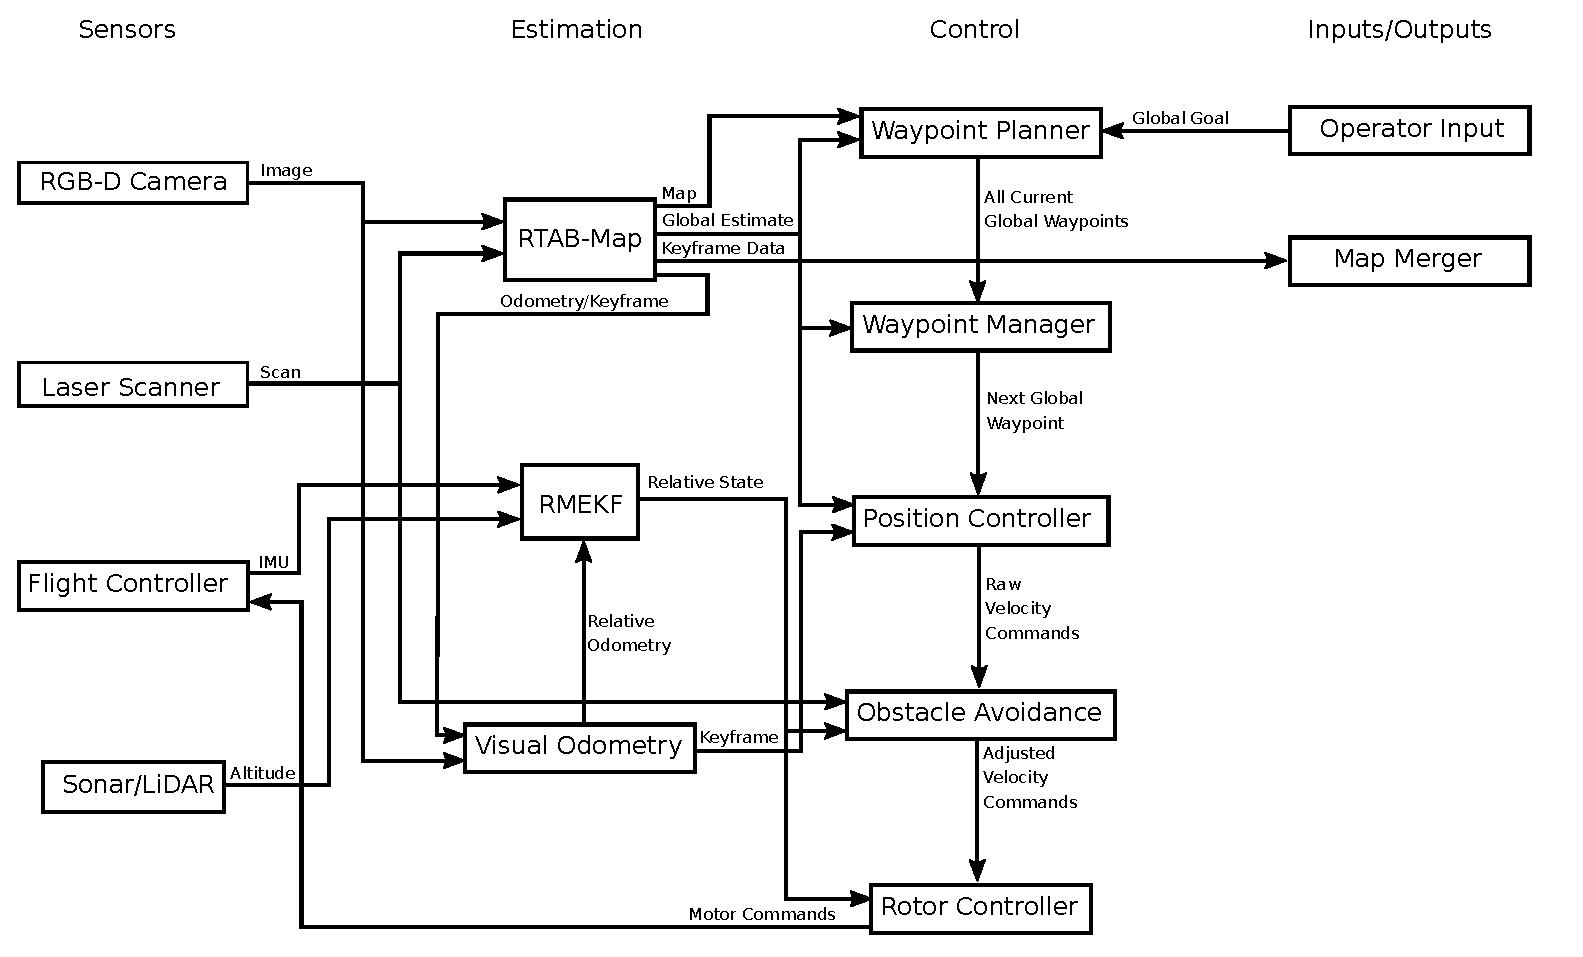
\includegraphics[width=1.0\linewidth]{rtab_relative_nav_network}
\caption{The network diagram of the relative navigation framework proposed in this paper}
\label{fig:rtab_network}
\end{figure*}


\subsubsection{Waypoints}


\subsection{Objective Functions}


\subsubsection{Maximize Coverage}

\begin{align}
  d_{\mathit{view},i} &= \max(\min(d_{\mathit{max}}, \min(d_{\mathit{obs},i})),d_{\mathit{min}}) \\
  i &= 0...m \nonumber
\end{align}
%

\begin{equation}\label{eq:coverage}%\nonumber
    \mathcal{C} = \alpha_{\mathit{cov}} \mathcal{C}_{\mathit{open}} + \left(1-\alpha_{\mathit{cov}})\right. \mathcal{C}_{\mathit{walls}},
\end{equation}

%%%%%%%%%%%%%%%%%%%%%%%%%%%%%%%%%%%%%%%%%%%%%%%%%%%%%%%%%%%%%%%%%%%%%%%%%%%%%%%%
\section{Planning}\label{Planning}



\subsection{Global Goal Following with Relative Estimation}



\subsection{Reactive Path Planning}

%%%%%%%%%%%%%%%%%%%%%%%%%%%%%%%%%%%%%%%%%%%%%%%%%%%%%%%%%%%%%%%%%%%%%%%%%%%%%%%%
\section{Map Merging}\label{merge}

%%%%%%%%%%%%%%%%%%%%%%%%%%%%%%%%%%%%%%%%%%%%%%%%%%%%%%%%%%%%%%%%%%%%%%%%%%%%%%%%
\section{Results and Discussion}\label{results}
The designer is required to set many parameters for the genetic algorithm to work as derived in \cite{Parkinson2019}. The parameters we used, along with parameters specific to our implementation, are outlined in Table \ref{tab:parameters}.

%%%%%%%%%%%%%%%%%%%%%%%%%%%%%%%%%%%%%%%%%%%%%%%%%%%%%%%%%%%%%%%%%%%%%%%%%%%%%%%%
\section{Conclusions}\label{conclusions}

We were able to successfully generate paths with sufficient coverage to generate a high-fidelity map of the environment that do not appear to meander too much for a single UAV. Future work on this project will include improving the loop closure implementation to allow the algorithm to explore the design space better without getting caught in local minima. This will enable more efficient paths to be created. We expect the need to use the paths generated with a lower level path planner that can dynamically change waypoints according to obstacles and other unmapped disparities. Finally we plan to test the paths generated both in high fidelity simulation as well as in hardware.

%%%%%%%%%%%%%%%%%%%%%%%%%%%%%%%%%%%%%%%%%%%%%%%%%%%%%%%%%%%%%%%%%%%%%%%%%%%%%%%%

\bibliographystyle{IEEEtran} % We choose the "plain" reference style
\bibliography{mapping_paper_2019}

\end{document}
